% =============================================================
%  CAPÍTULO III — METODOLOGÍA
% =============================================================

\section{Marco de fases de desarrollo del proyecto tecnológico}

El desarrollo del proyecto tecnológico Kiddy Quiz se estructuró en torno a tres etapas principales y secuenciales: la obtención de requisitos, el desarrollo de la aplicación, y las pruebas e implementación. Esta distribución metodológica está alineada con la propuesta de Beck y Andres~\cite{beck2004xp}, la cual promueve la presentación de prototipos o incrementos funcionales para la visualización temprana de las interfaces y la evaluación continua de las funcionalidades a lo largo del ciclo de vida del proyecto.

Para ejecutar este flujo de trabajo, se adoptaron las prácticas de la Programación Extrema (XP), adaptadas al contexto específico del proyecto \cite{beck2004xp,dyba2008agile}. Al tratarse de un desarrollo individual, las prácticas colaborativas de XP se reorientaron hacia la autodisciplina y la revisión personal del código, mientras que la evaluación continua con los expertos se estructuró en ciclos de retroalimentación planificados, ajustados a la disponibilidad de los actores educativos involucrados. De esta manera, la obtención de requisitos se gestionó mediante el \textit{Planning Game} y la construcción de Historias de Usuario; el desarrollo de la aplicación se centró en el ciclo de Desarrollo Dirigido por Pruebas (TDD), la refactorización y el diseño simple; y las pruebas e implementación se basaron en la entrega de lanzamientos pequeños para la validación continua del sistema con los usuarios finales \cite{dyba2008agile,shrivastava2021xpreview}.

La elección de XP como metodología de desarrollo responde a su idoneidad documentada para contextos donde los requisitos pueden evolucionar y donde la participación activa del usuario final es fundamental para garantizar la pertinencia pedagógica del producto \cite{beck2004xp}. La revisión sistemática de Dybå y Dingsøyr \cite{dyba2008agile} confirma que XP produce mejoras consistentes en calidad de código, satisfacción del cliente y capacidad de respuesta ante cambios, ventajas que resultan críticas en el desarrollo de software educativo orientado a usuarios con necesidades específicas.

\begin{figure}[H]
  \centering
  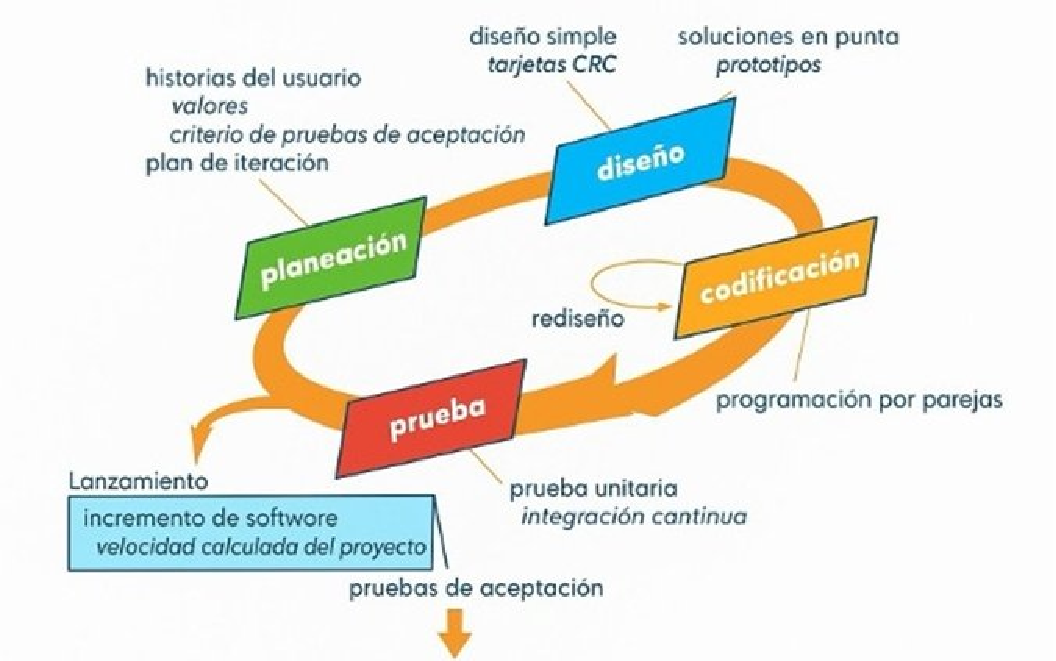
\includegraphics[width=0.85\textwidth]{QuizKidsV2/figuras/fig01_metodologia_xp.pdf}
  \caption{Metodología XP aplicada al desarrollo de Kiddy Quiz.}
  \label{fig:xp}
\end{figure}
\fuenteautor

\subsection{Obtención de requisitos}

La fase de obtención de requisitos tuvo como objetivo principal comprender de manera integral las necesidades pedagógicas, cognitivas y funcionales asociadas a la evaluación por competencias en Matemáticas en el nivel de educación básica elemental, superando un enfoque limitado a aspectos exclusivamente técnicos \cite{evans2020cbe}. Para ello, se aplicó el Juego de Planificación o \textit{Planning Game}, práctica central de la metodología XP, adaptada al contexto académico y a las características de un proyecto de titulación individual.

La interacción con los usuarios finales se estructuró mediante ciclos de comunicación planificados con siete expertos vinculados al contexto educativo: cinco docentes de educación básica elemental con experiencia en evaluación por competencias matemáticas y dos psicopedagogos vinculados al ámbito universitario, quienes asumieron el rol de \textit{On-site Customer} en la metodología XP. Este enfoque permitió establecer un canal de retroalimentación constante y asegurar que los requerimientos del sistema respondieran a necesidades reales del contexto educativo ecuatoriano \cite{velezvelez2024curriculo}.

\subsubsection{Análisis preliminar y contextual}

Como punto de partida, se llevó a cabo un análisis preliminar orientado a evaluar la viabilidad del proyecto y a delimitar su alcance funcional. Las entrevistas a los docentes se realizaron de manera presencial en sus respectivos hogares, con un carácter formal orientado a recopilar información detallada sobre sus prácticas evaluativas, los desafíos enfrentados en la enseñanza de Matemáticas y las limitaciones de los métodos tradicionales de evaluación \cite{velezvelez2024curriculo,niss2019math}. En contraste, las entrevistas a los psicopedagogos se llevaron a cabo de forma presencial en la Universidad Técnica Estatal de Quevedo, bajo un enfoque no estructurado destinado a orientar el diseño pedagógico e inclusivo del sistema desde una perspectiva especializada.

Todas las entrevistas fueron individuales y previo a su ejecución se obtuvo el consentimiento informado por escrito de los participantes. En el caso de los docentes, se realizó el registro mediante grabaciones de audio y toma de notas; con los psicopedagogos se empleó únicamente registro escrito.

\subsubsection{Ejecución del Juego de Planificación}

El Juego de Planificación se aplicó mediante entrevistas semiestructuradas apoyadas en una guía de diez preguntas previamente definida (véase Anexos). Cada entrevista tuvo una duración aproximada de 40 minutos y se enfocó en cuatro ejes principales: la experiencia docente en la enseñanza de Matemáticas, los desafíos asociados a la evaluación de competencias matemáticas, el uso de herramientas digitales en los procesos evaluativos y las expectativas respecto a una aplicación orientada a evaluaciones por competencias.

Durante el desarrollo de las entrevistas, se presentaron interfaces preliminares del sistema como prototipos funcionales, obtenidos de la revisión de aplicaciones existentes como \textit{Kahoot!}, \textit{Quizizz}, \textit{Nearpod}, \textit{Socrative} y \textit{ClassDojo}, lo cual permitió ``amplificar el aprendizaje'', una práctica característica de XP que facilita la comprensión de los requisitos y promueve una retroalimentación más precisa por parte de los expertos \cite{beck2004xp}.

\subsubsection{Definición y documentación de Historias de Usuario}

A partir de la información recopilada, se definieron y documentaron las historias de usuario como principal insumo para la planificación del desarrollo. En total se elaboraron 27 historias de usuario, redactadas desde una perspectiva centrada principalmente en el rol del docente como usuario responsable de la gestión de evaluaciones y del seguimiento del progreso académico de los estudiantes.

Cada historia de usuario incluyó criterios de aceptación de carácter pedagógico definidos en conjunto con los expertos, entre los que se destacan: el diseño intuitivo y visualmente atractivo para los estudiantes, la incorporación de formatos de preguntas variados y la disponibilidad de herramientas para el seguimiento detallado de los resultados \cite{evans2020cbe,vlachogianni2022sus}. La priorización de las historias de usuario permitió organizar el trabajo en incrementos funcionales, asegurando la entrega progresiva de valor conforme a los principios de XP.

\subsection{Desarrollo de la aplicación}

La fase de desarrollo de la aplicación constituyó el núcleo del proyecto, en la cual se materializaron los requerimientos definidos durante la primera etapa. Su ejecución siguió los principios de XP, priorizando ciclos de desarrollo cortos, la simplicidad en el diseño y la entrega continua de funcionalidades completas y operativas \cite{dyba2008agile}.

Al ser un desarrollo individual, la práctica de \textit{Pair Programming} fue adaptada a un enfoque de autoevaluación y revisión crítica del código mediante la técnica del ``patito de goma'' —que consiste en explicar en voz alta la lógica del código desarrollado— y mediante sesiones periódicas de revisión con el director del proyecto, lo que permitió identificar inconsistencias, errores lógicos y oportunidades de mejora. El control de versiones se gestionó mediante un repositorio público en GitHub, lo que facilitó el seguimiento de cambios y la organización del historial de incrementos funcionales.

\subsubsection{Generación y adaptación de modelos}

Desde la perspectiva del docente, se implementaron funcionalidades orientadas a la gestión de clases, evaluaciones y preguntas, la administración de estudiantes y la generación de reportes analíticos. Desde la perspectiva del estudiante, el sistema permite el acceso a clases y evaluaciones asignadas, la visualización del progreso académico y la participación en actividades de refuerzo asistidas por IA. Durante el desarrollo se priorizó el principio de diseño simple, evitando el modelado exhaustivo previo y permitiendo que la estructura del sistema evolucionara en función de las necesidades reales del proyecto, en concordancia con los valores de XP \cite{beck2004xp,shrivastava2021xpreview}.

\subsubsection{Generación de pruebas y software (TDD)}

La implementación del software se realizó aplicando de manera parcial el enfoque de Desarrollo Dirigido por Pruebas (TDD), como adaptación de la metodología XP, equilibrando las exigencias metodológicas con la viabilidad de un proyecto individual con restricciones de tiempo \cite{dyba2008agile}. En los módulos críticos del sistema ---la gestión de clases, el cálculo de resultados y el seguimiento del progreso académico--- se siguió el ciclo característico de TDD: se definieron pruebas automatizadas que fallaban, se implementó el código mínimo necesario para superarlas y, finalmente, se realizaron procesos de refactorización para mejorar la calidad y mantenibilidad del código.

Las pruebas desarrolladas incluyeron pruebas unitarias y de integración, enfocadas en los servicios y en la validación de la interacción entre el \textit{frontend} y el \textit{backend}. Para su ejecución se empleó el \textit{framework} Jest, integrado al entorno de desarrollo Visual Studio Code, en un proyecto construido con NestJS para el \textit{backend} y Angular para el \textit{frontend}, utilizando Node.js como entorno de ejecución, npm como gestor de dependencias, GitHub para el control de versiones y PostgreSQL como sistema de gestión de base de datos.

\subsubsection{Refactorización continua del código}

La refactorización se aplicó como una práctica constante a lo largo de los ciclos de desarrollo, orientada a mejorar la legibilidad, estructura y mantenibilidad del código sin alterar su comportamiento funcional \cite{beck2004xp}. Esta actividad permitió reducir la complejidad de los módulos implementados, eliminar duplicación de código y adaptar la arquitectura del sistema a medida que se incorporaban nuevas funcionalidades. La refactorización no se concibió como una fase aislada, sino como una actividad iterativa que acompañó a cada incremento funcional, contribuyendo a mantener la calidad y estabilidad del sistema conforme evolucionó su implementación.

\subsubsection{Stack tecnológico y versiones utilizadas}

Con el propósito de garantizar la reproducibilidad del entorno de desarrollo y facilitar
la replicación del proyecto por parte de investigadores o desarrolladores futuros,
en la Tabla~\ref{tab:versiones} se detallan las tecnologías empleadas y sus versiones
específicas. El criterio de selección de versiones fue el uso de la versión estable
más reciente disponible al inicio del desarrollo del proyecto \cite{dyba2008agile,beck2004xp}.

\begin{table}[H]
\centering
\caption{Stack tecnológico y versiones del proyecto Kiddy Quiz.}
\label{tab:versiones}
\footnotesize
\renewcommand{\arraystretch}{1.3}
\begin{tabularx}{\textwidth}{|p{3.5cm}|p{2.2cm}|p{2.2cm}|X|}
\hline
\rowcolor{headblue}
\textbf{Tecnología} & \textbf{Versión} & \textbf{Rol} & \textbf{Propósito en el proyecto} \\\hline
Angular & 19.x & \textit{Frontend} & Framework para la construcción de la interfaz de usuario y componentes interactivos \\\hline
NestJS & 11.x & \textit{Backend} & Framework para la lógica de negocio, gestión de rutas API REST y protocolos de seguridad \\\hline
PostgreSQL & 17.x & Base de datos & Motor de base de datos relacional para el almacenamiento estructurado de evaluaciones, usuarios y resultados \\\hline
Node.js & 22 LTS & Entorno de ejecución & Plataforma de ejecución del servidor \textit{backend} (codename \textit{Jod}) \\\hline
npm & 10.x & Gestor de paquetes & Administración de dependencias del \textit{frontend} y \textit{backend} \\\hline
Jest & 29.x & Pruebas & \textit{Framework} de pruebas unitarias e integración para los módulos críticos del sistema \\\hline
TypeScript & 5.x & Lenguaje & Superset de JavaScript con tipado estático utilizado en Angular y NestJS \\\hline
Cloudinary & API v2 & Multimedia & Almacenamiento y gestión optimizada de recursos multimedia (imágenes, GIFs) \\\hline
Gemini 2.5 Flash & API v1beta & Inteligencia artificial & Generación de retroalimentación motivacional y recomendaciones pedagógicas \\\hline
JSON Web Token (JWT) & 9.x & Seguridad & Autenticación y control de acceso basado en roles (docente/estudiante) \\\hline
GitHub & --- & Control de versiones & Repositorio público para gestión del código fuente con dos ramas de trabajo \\\hline
Visual Studio Code & 1.9x & IDE & Entorno de desarrollo integrado con extensiones para Angular, NestJS y Jest \\\hline
\end{tabularx}
\end{table}
\fuenteautor

\subsection{Pruebas e implementación}

La fase de pruebas e implementación se orientó a la validación progresiva del sistema y a la verificación de que las funcionalidades desarrolladas respondieran a los requisitos definidos durante la planificación. En concordancia con los principios de XP, esta etapa se centró en la evaluación continua del software mediante incrementos funcionales \cite{dyba2008agile,shrivastava2021xpreview}.

\subsubsection{Implementación del software}

La implementación del software se gestionó mediante un repositorio de control de versiones en GitHub. El desarrollo se realizó de manera iterativa: en una primera fase se estableció la estructura base del sistema, definiendo la arquitectura general, el modelo de base de datos y los módulos relacionados con la autenticación, la gestión de usuarios, las evaluaciones y los reportes. Posteriormente, en el \textit{frontend} se priorizó la implementación completa del flujo de evaluación desde la perspectiva del estudiante, asegurando la coherencia entre las funcionalidades y la experiencia de uso. Cada versión del software correspondió a un incremento funcional asociado a una historia de usuario previamente priorizada; dichos incrementos fueron revisados por el director del proyecto y por docentes, lo que facilitó la identificación temprana de ajustes necesarios y la consolidación progresiva del sistema.

\subsubsection{Evaluación del entregable}

La evaluación de los entregables se realizó de manera iterativa, considerando tanto pruebas de funcionamiento como pruebas de usabilidad. Las pruebas funcionales se orientaron a verificar el correcto cumplimiento de los requerimientos definidos. Paralelamente, con la participación de cinco docentes de educación básica elemental, se llevaron a cabo pruebas de usabilidad mediante observación directa y la aplicación del \textit{System Usability Scale} (SUS) y el \textit{Technology Acceptance Model} (TAM) \cite{brooke1996sus,davis1989tam,vlachogianni2022sus}. Estas pruebas permitieron analizar la interacción de los usuarios con la aplicación, identificar dificultades en la navegación y evaluar la claridad de las interfaces, especialmente desde la perspectiva del uso infantil.

\subsubsection{Pruebas de aceptación}

Las pruebas de aceptación constituyeron la etapa final de validación del sistema, orientada a verificar que el software desarrollado cumpliera con las expectativas y necesidades de los expertos en evaluación por competencias. La evaluación final contrastó las funcionalidades implementadas con los criterios de aceptación definidos en las historias de usuario. La retroalimentación obtenida confirmó la pertinencia del enfoque adoptado, destacándose el diseño intuitivo de la aplicación, la claridad en la presentación de las evaluaciones y la utilidad de las herramientas de seguimiento del progreso académico.

\subsubsection*{Despliegue en producción}

Una vez superadas las pruebas de aceptación, el sistema fue desplegado en el
servidor institucional de la Universidad Técnica Estatal de Quevedo y se encuentra
accesible de forma pública en la URL:
\begin{center}
  \url{https://aplicaciones.uteq.edu.ec/kiddquiz}
\end{center}

El despliegue se realizó configurando el \textit{backend} (NestJS~11 sobre Node.js~22~LTS)
como un proceso persistente gestionado por el administrador de procesos PM2, mientras
que el \textit{frontend} (Angular~19) fue compilado en modo de producción mediante el
comando \texttt{ng build -{}-configuration=production} y servido a través del servidor
web del entorno institucional. La base de datos PostgreSQL~17 fue configurada en el
mismo servidor, con acceso restringido por credenciales y sin exposición directa
al exterior. Las variables de entorno sensibles ---incluyendo las claves de API de
Gemini, las credenciales de Cloudinary y el secreto JWT--- fueron configuradas
directamente en el entorno del servidor y no se incluyen en el repositorio público,
en cumplimiento del requerimiento no funcional RNF-02 de seguridad y protección de datos.

Para reproducir el despliegue local del proyecto, un investigador debe:

\begin{enumerate}[leftmargin=*, label=\arabic*.]
  \item Clonar el repositorio público desde GitHub.
  \item Instalar las dependencias con \texttt{npm install} tanto en el directorio del \textit{frontend} como del \textit{backend}.
  \item Configurar un archivo \texttt{.env} con las variables de entorno requeridas (detalladas en el archivo \texttt{README.md} del repositorio).
  \item Ejecutar las migraciones de la base de datos con el comando correspondiente de TypeORM.
  \item Iniciar el \textit{backend} con \texttt{npm run start:dev} y el \textit{frontend} con \texttt{ng serve}.
\end{enumerate}

\subsection{Evaluación de la aplicación}
\subsubsection*{Criterios de selección de participantes}

La evaluación se realizó con una muestra intencional no probabilística de
veinte participantes, seleccionados con base en criterios de inclusión y
exclusión definidos previamente \cite{vlachogianni2022sus}.

Para el \textbf{grupo de estudiantes} ($N = 15$), los criterios de inclusión fueron: pertenecer al nivel de educación básica elemental (2.°, 3.° o 4.° año de EGB), tener entre 6 y 9 años de edad, contar con experiencia mínima en el uso de dispositivos con pantalla táctil o ratón, y disponer del consentimiento informado firmado por el representante legal. Se excluyeron estudiantes con discapacidades visuales o motoras severas que impidieran la interacción autónoma con la interfaz.

Para el \textbf{grupo de docentes} ($N = 5$), los criterios de inclusión fueron: ejercer docencia activa en el área de Matemáticas en el nivel básico elemental, tener al menos un año de experiencia en procesos de evaluación por competencias y haber participado previamente en la fase de levantamiento de requisitos del proyecto. Se excluyeron docentes sin acceso a computadora durante la sesión
de evaluación.

Las sesiones de evaluación se realizaron de manera individual, con una duración promedio de 45 minutos por participante, en entornos controlados que garantizaron la interacción directa con la versión de producción del sistema desplegada en \url{https://aplicaciones.uteq.edu.ec/kiddquiz}.

Para la recolección de información se emplearon cuatro instrumentos complementarios. En primer lugar, una \textbf{guía de entrevista semiestructurada} de diez preguntas aplicada a los docentes, disponible en el Anexo~A, organizada en cuatro ejes: experiencia docente en Matemáticas, desafíos en la evaluación por competencias, uso de herramientas digitales y expectativas sobre la aplicación. En segundo lugar, una \textbf{rúbrica de observación directa} utilizada durante las sesiones de prueba con usuarios, disponible en el Anexo~B. En tercer lugar, el \textbf{cuestionario \textit{System Usability Scale} (SUS)} en su versión adaptada al español de diez ítems con escala Likert de 1 a 5, cuya puntuación se calcula mediante la fórmula estándar de Brooke \cite{brooke1996sus} (véase Anexo~C). Finalmente, el \textbf{cuestionario del Modelo de Aceptación Tecnológica (TAM)} en su versión de doce ítems agrupados en tres dimensiones ---Utilidad Percibida (PU), Facilidad de Uso Percibida (PEOU) e Intención de Uso (IU)---, con escala Likert de 1 a 5 \cite{davis1989tam} (véase Anexo~D). Todos los participantes firmaron el formato de consentimiento informado disponible en el Anexo~E previo a la aplicación
de cualquier instrumento.

Para la recolección de información se emplearon una rúbrica de observación, apuntes de campo y los cuestionarios estandarizados SUS y TAM \cite{brooke1996sus,davis1989tam}. Estos instrumentos permitieron obtener datos cualitativos y cuantitativos orientados a medir la eficiencia, efectividad y satisfacción de los usuarios durante la interacción con el sistema. En el caso de los estudiantes, se puso especial énfasis en la facilidad de uso, el carácter intuitivo del diseño y el nivel de interacción generado por las actividades propuestas. Por su parte, los docentes evaluaron la utilidad de las herramientas de gestión, el seguimiento del progreso académico y el análisis de resultados. La información recopilada fue sistematizada para su posterior análisis, cuyos resultados cuantitativos y cualitativos se presentan en el Capítulo~IV.

\section{Cronograma}

Para alcanzar los objetivos del proyecto, se presenta en la Figura~\ref{fig:cronograma} el cronograma de 32 semanas que detalla las actividades realizadas a lo largo del proceso de desarrollo, abarcando desde el análisis y estructuración del tema hasta la entrega de la documentación correspondiente al trabajo de integración curricular. En concordancia con la naturaleza iterativa de la metodología XP, el cronograma mantuvo un enfoque flexible: las fechas de finalización de ciertos módulos experimentaron ligeros ajustes para incorporar correcciones, mejoras de usabilidad y refactorizaciones derivadas de la retroalimentación continua, garantizando la calidad del producto final dentro del plazo estipulado.

% Requiere en el preámbulo:
% \usepackage{tikz}
% \usepackage{xcolor}

\begin{figure}[H]
\centering
\caption{Cronograma de actividades del proyecto Kiddy Quiz.}
\label{fig:cronograma}
\resizebox{\textwidth}{!}{%
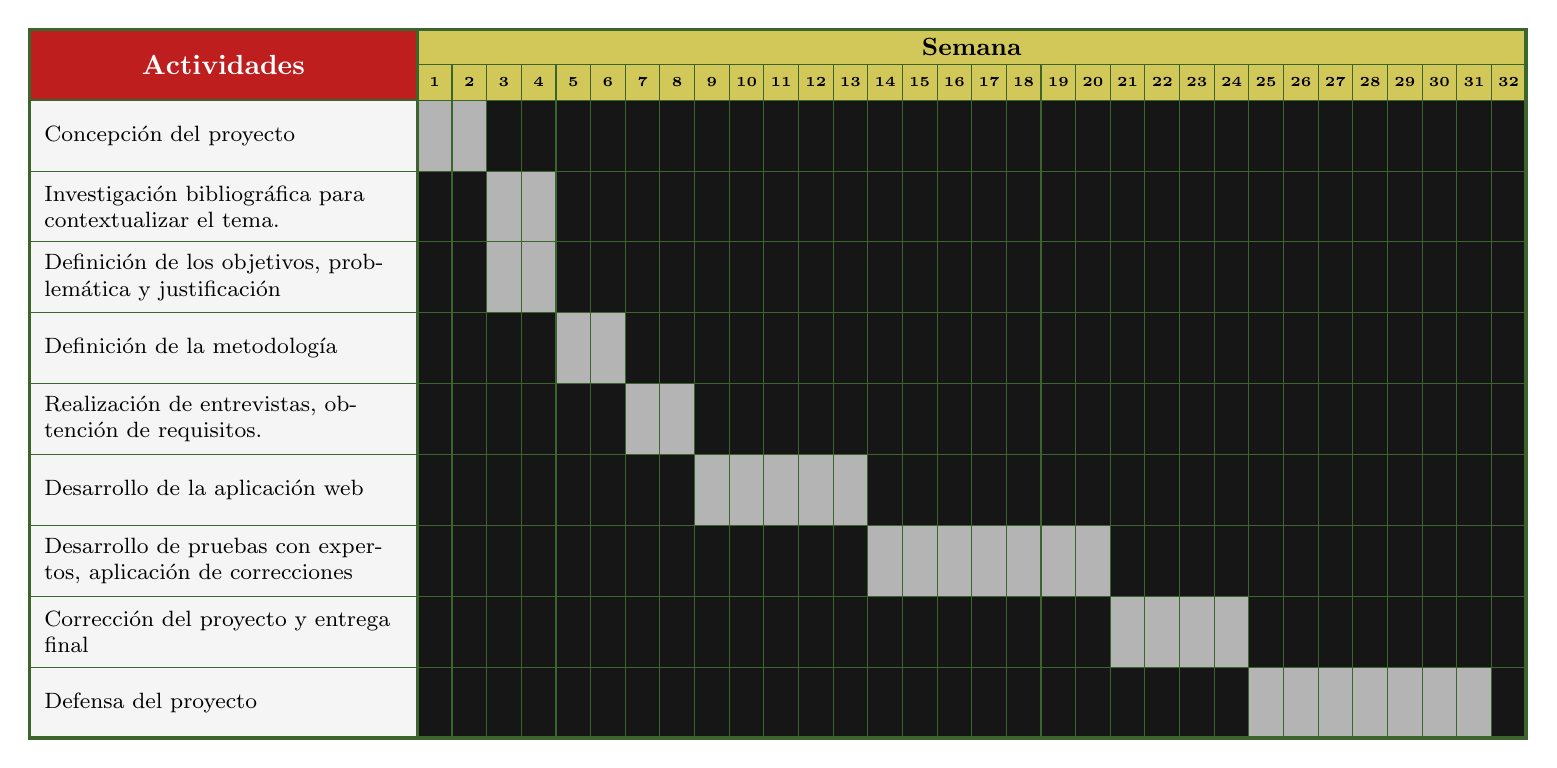
\begin{tikzpicture}[x=0.44cm, y=0.9cm]

\definecolor{celdag}{RGB}{180,180,180}
\definecolor{rojoenc}{RGB}{190,30,30}
\definecolor{amarenc}{RGB}{210,200,90}
\definecolor{fondoN}{RGB}{22,22,22}
\definecolor{verdef}{RGB}{60,100,45}
\definecolor{blancof}{RGB}{245,245,245}

\def\NC{32}
\def\AW{11.2}

% Fondo negro zona grid
\fill[fondoN] (0,-10) rectangle (\NC,-1);

% Header "Semana"
\fill[amarenc] (0,-0.5) rectangle (\NC,0);
\draw[verdef,thin] (0,-0.5) rectangle (\NC,0);
\node[font=\bfseries\small] at (16,-0.25) {Semana};

% Números 1-32
\foreach \s in {1,...,32}{
  \fill[amarenc] (\s-1,-1) rectangle (\s,-0.5);
  \draw[verdef,thin] (\s-1,-1) rectangle (\s,-0.5);
  \node[font=\tiny\bfseries] at (\s-0.5,-0.75) {\s};
}

% Encabezado "Actividades"
\fill[rojoenc] (-\AW,-1) rectangle (0,0);
\draw[verdef,thick] (-\AW,-1) rectangle (0,0);
\node[font=\bfseries\normalsize, text=white] at (-\AW/2,-0.5) {Actividades};

% Fondo blanco columna actividades
\fill[blancof] (-\AW,-10) rectangle (0,-1);

% === CELDAS ACTIVAS (gris) ===
\foreach \s in {1,2}{       \fill[celdag] (\s-1,-2)  rectangle (\s,-1);  }
\foreach \s in {3,4}{       \fill[celdag] (\s-1,-3)  rectangle (\s,-2);  }
\foreach \s in {3,4}{       \fill[celdag] (\s-1,-4)  rectangle (\s,-3);  }
\foreach \s in {5,6}{       \fill[celdag] (\s-1,-5)  rectangle (\s,-4);  }
\foreach \s in {7,8}{       \fill[celdag] (\s-1,-6)  rectangle (\s,-5);  }
\foreach \s in {9,...,13}{  \fill[celdag] (\s-1,-7)  rectangle (\s,-6);  }
\foreach \s in {14,...,20}{ \fill[celdag] (\s-1,-8)  rectangle (\s,-7);  }
\foreach \s in {21,...,24}{ \fill[celdag] (\s-1,-9)  rectangle (\s,-8);  }
\foreach \s in {25,...,31}{ \fill[celdag] (\s-1,-10) rectangle (\s,-9);  }

% === GRILLA ===
\foreach \r in {1,...,10}{ \draw[verdef,thin] (0,-\r)    -- (\NC,-\r);  }
\foreach \s in {0,...,32}{ \draw[verdef,thin] (\s,-1)    -- (\s,-10);   }
\foreach \r in {1,...,10}{ \draw[verdef,thin] (-\AW,-\r) -- (0,-\r);    }

% === TEXTOS ===
\node[font=\footnotesize, align=left, text width=4.4cm, anchor=west]
  at (-\AW+0.15,-1.5) {Concepción del proyecto};
\node[font=\footnotesize, align=left, text width=4.4cm, anchor=west]
  at (-\AW+0.15,-2.5) {Investigación bibliográfica para contextualizar el tema.};
\node[font=\footnotesize, align=left, text width=4.4cm, anchor=west]
  at (-\AW+0.15,-3.5) {Definición de los objetivos, problemática y justificación};
\node[font=\footnotesize, align=left, text width=4.4cm, anchor=west]
  at (-\AW+0.15,-4.5) {Definición de la metodología};
\node[font=\footnotesize, align=left, text width=4.4cm, anchor=west]
  at (-\AW+0.15,-5.5) {Realización de entrevistas, obtención de requisitos.};
\node[font=\footnotesize, align=left, text width=4.4cm, anchor=west]
  at (-\AW+0.15,-6.5) {Desarrollo de la aplicación web};
\node[font=\footnotesize, align=left, text width=4.4cm, anchor=west]
  at (-\AW+0.15,-7.5) {Desarrollo de pruebas con expertos, aplicación de correcciones};
\node[font=\footnotesize, align=left, text width=4.4cm, anchor=west]
  at (-\AW+0.15,-8.5) {Corrección del proyecto y entrega final};
\node[font=\footnotesize, align=left, text width=4.4cm, anchor=west]
  at (-\AW+0.15,-9.5) {Defensa del proyecto};

% === BORDE EXTERIOR ===
\draw[verdef,very thick] (-\AW,-10) rectangle (\NC,0);
\draw[verdef,very thick] (0,-10) -- (0,0);

\end{tikzpicture}%
}
\fuenteautor
\end{figure}


\section{Recursos, presupuesto y financiamiento}

En la Tabla~\ref{tab:presupuesto} se presenta el presupuesto que cubre los recursos utilizados para el desarrollo de Kiddy Quiz, detallando los insumos, herramientas tecnológicas y servicios empleados a lo largo del proyecto. El costo total refleja inversiones en hardware disponible, software de código abierto y gratuito, y recursos humanos especializados del ámbito universitario, lo que evidencia la viabilidad económica de la propuesta.

\begin{table}[H]
\centering
\caption{Presupuesto del proyecto Kiddy Quiz.}
\label{tab:presupuesto}
\footnotesize
\renewcommand{\arraystretch}{1.4}
\begin{tabularx}{\textwidth}{|>{\bfseries}p{2.2cm}|p{2.4cm}|p{2.2cm}|X|p{2cm}|r|}
\hline
\rowcolor{headblue}
\textbf{Tipo} &
\textbf{Categoría} &
\textbf{Recurso} &
\textbf{Descripción} &
\textbf{Fuente} &
\textbf{Precio (\$)} \\\hline

\multirow{3}{2.2cm}{\centering Recursos disponibles} &
\multirow{3}{2.4cm}{\centering Infraestructura} &
Equipo &
Laptop &
Personal &
150{,}50 \\\cline{3-6}

& &
Equipo &
Teléfono móvil &
Personal &
45{,}00 \\\cline{3-6}

& &
Vehículo &
Para el traslado a la entrevista. &
Personal &
5{,}00 \\\hline

\multirow{3}{2.2cm}{\centering Recursos necesarios} &
\multirow{2}{2.4cm}{\centering Tecnologías de desarrollo} &
Visual Studio Code &
Editor de código fuente. &
Microsoft &
0{,}00 \\\cline{3-6}

& &
PostgreSQL &
Base de datos de código abierto. &
Google &
0{,}00 \\\cline{2-6}

&
Recursos humanos &
Profesionales en el área educativa &
Expertos en el área educativa, especialmente que tengan experiencia en el desarrollo o implementación de las evaluaciones por competencias. &
Universidad &
0{,}00 \\\hline

\end{tabularx}
\end{table}
\fuenteautor

\section{Instrumentos para el seguimiento y control}

El seguimiento y control del proyecto constituyeron actividades fundamentales para garantizar el cumplimiento de los objetivos planteados, el uso adecuado de los recursos disponibles y el desarrollo ordenado de las fases definidas en la metodología \cite{beck2004xp,dyba2008agile}.

La gestión y seguimiento de tareas se realizó mediante Microsoft Excel, herramienta principal de planificación en la que las actividades se organizaron en tres estados: pendiente, en proceso y completado. Complementariamente, se elaboró un diagrama de Gantt con tiempos estimados de inicio y finalización para cada tarea.

El control de versiones del software se llevó a cabo mediante la plataforma GitHub, utilizando un repositorio público disponible en \url{https://github.com/JCabrera07/KiddyQuiz}\footnote{En caso de que la URL cambie, el sistema puede ser también consultado en su versión de producción en \url{https://aplicaciones.uteq.edu.ec/kiddquiz}.},
el cual permitió gestionar de forma ordenada los cambios realizados en el código fuente. Durante el desarrollo se emplearon dos ramas de trabajo (\texttt{main} y \texttt{develop}), dado que el proyecto se desarrolló desde dos computadoras con sistemas operativos distintos (Windows y macOS). Esta estrategia facilitó la integración del código, la sincronización de los avances y la recuperación de versiones anteriores cuando fue necesario, en concordancia con la práctica de integración continua de XP \cite{beck2004xp}.

Para la gestión documental se utilizó de manera complementaria el almacenamiento local y Google Drive, donde se organizaron y resguardaron las entrevistas, los formatos de consentimiento informado, los anexos, las capturas de pantalla de las interfaces del sistema y la documentación técnica. La comunicación y retroalimentación con los docentes expertos se realizó principalmente de forma presencial y a través de la aplicación WhatsApp, canal que permitió una interacción ágil sin necesidad de reuniones formales programadas.

En lo referente al seguimiento técnico, se implementaron pruebas automatizadas con el \textit{framework} Jest, que permitieron verificar el funcionamiento de distintos componentes del sistema, detectar errores en ciertos \textit{endpoints} ---especialmente los relacionados con el seguimiento del progreso del estudiante y la retroalimentación generada por la IA--- y registrar observaciones para la reorganización de tareas y la corrección del código. Para la elaboración de la documentación formal y la presentación de resultados se empleó la suite Microsoft Office (Word, Excel y PowerPoint).

Los riesgos identificados durante el desarrollo ---limitaciones de tiempo, disponibilidad de los expertos, complejidad técnica y dificultades de implementación--- se gestionaron mediante la reorganización de tareas y el ajuste de la planificación, permitiendo continuar el desarrollo de manera controlada y conforme a los objetivos establecidos.

\section{Indicadores de evaluación}
\label{sec:indicadores}

En esta sección se describen los indicadores utilizados para verificar el cumplimiento de las especificaciones del proyecto tecnológico y para analizar de manera crítica los resultados obtenidos durante su desarrollo \cite{vlachogianni2022sus,brooke1996sus,davis1989tam}. Estos indicadores permitieron validar que el sistema responde al problema planteado, cumple con los requisitos definidos y satisface las necesidades de los usuarios finales. Las actividades de verificación y validación se ejecutaron a lo largo de las distintas fases del proyecto, considerando el cumplimiento del cronograma, el alcance funcional, la calidad del sistema, la usabilidad, la aceptación tecnológica, el rendimiento técnico, la seguridad básica y el nivel de innovación educativa incorporado.

\begin{table}[H]
\centering
\caption{Indicador de cumplimiento de plazos.}
\label{tab:ind_plazos}
\footnotesize
\renewcommand{\arraystretch}{1.25}
\begin{tabularx}{\textwidth}{|>{\bfseries}p{3.2cm}|X|}
\hline
\rowcolor{headblue}\multicolumn{2}{|c|}{\textbf{Cumplimiento de plazos}}\\\hline
Descripción & Mide la capacidad del proyecto para cumplir con los tiempos establecidos para el desarrollo de las actividades y fases definidas en el cronograma. \\\hline
Medición & Se estableció un cronograma inicial ajustado iterativamente durante el desarrollo. Se utilizaron diagramas de Gantt y listas de tareas en Microsoft Excel, organizadas en los estados ``Pendiente'', ``En proceso'' y ``Completado''. Se compararon las fechas planificadas con las fechas reales de finalización. \\\hline
Criterios de éxito & Se consideró satisfactorio si al menos el 90\,\% de las tareas se completaron dentro de los plazos ajustados, aceptando retrasos leves no críticos. \\\hline
\end{tabularx}
\end{table}
\fuenteautor

\begin{table}[H]
\centering
\caption{Indicador de cumplimiento del alcance del proyecto.}
\label{tab:ind_alcance}
\footnotesize
\renewcommand{\arraystretch}{1.25}
\begin{tabularx}{\textwidth}{|>{\bfseries}p{3.2cm}|X|}
\hline
\rowcolor{headblue}\multicolumn{2}{|c|}{\textbf{Cumplimiento del alcance}}\\\hline
Descripción & Evalúa el grado de cumplimiento de los objetivos y requisitos funcionales definidos para el sistema. \\\hline
Medición & Se verificó la implementación de las 29 historias de usuario definidas durante la fase de análisis y se realizó una validación funcional de los módulos principales del sistema. \\\hline
Criterios de éxito & El indicador se considera satisfactorio si todas las historias de usuario fueron implementadas y las funcionalidades principales operan correctamente. \\\hline
\end{tabularx}
\end{table}
\fuenteautor

\begin{table}[H]
\centering
\caption{Indicador de calidad del producto.}
\label{tab:ind_calidad}
\footnotesize
\renewcommand{\arraystretch}{1.25}
\begin{tabularx}{\textwidth}{|>{\bfseries}p{3.2cm}|X|}
\hline
\rowcolor{headblue}\multicolumn{2}{|c|}{\textbf{Calidad del sistema}}\\\hline
Descripción & Mide el nivel de calidad del sistema en términos de estabilidad, funcionalidad y ausencia de errores críticos. \\\hline
Medición & Se realizaron pruebas unitarias, de integración y funcionales manuales con el \textit{framework} Jest. Las pruebas se ejecutaron de forma parcial antes de la evaluación con usuarios y sus resultados se registraron para orientar la refactorización. \\\hline
Criterios de éxito & El sistema se considera de calidad adecuada si no presenta errores críticos que afecten su funcionamiento principal durante las sesiones de evaluación con usuarios reales. \\\hline
\end{tabularx}
\end{table}
\fuenteautor

\begin{table}[H]
\centering
\caption{Indicador de usabilidad y satisfacción del usuario.}
\label{tab:ind_sus}
\footnotesize
\renewcommand{\arraystretch}{1.25}
\begin{tabularx}{\textwidth}{|>{\bfseries}p{3.2cm}|X|}
\hline
\rowcolor{headblue}\multicolumn{2}{|c|}{\textbf{Nivel de satisfacción del usuario}}\\\hline
Descripción & Evalúa la percepción de los usuarios finales sobre la facilidad de uso y la experiencia general del sistema, aplicado a quince estudiantes de educación básica elemental y cinco docentes. \\\hline
Medición & Se aplicó el cuestionario SUS (\textit{System Usability Scale}) \cite{brooke1996sus}, instrumento con amplia validación empírica en tecnología educativa \cite{vlachogianni2022sus}. Se complementó con retroalimentación cualitativa recopilada durante las sesiones de evaluación mediante rúbricas de observación. \\\hline
Criterios de éxito & El indicador se considera satisfactorio si la puntuación SUS alcanza o supera el valor de referencia de 68 puntos, umbral establecido como mínimo aceptable en la industria del software \cite{brooke1996sus}. \\\hline
\end{tabularx}
\end{table}
\fuenteautor

\begin{table}[H]
\centering
\caption{Indicador de aceptación tecnológica (TAM).}
\label{tab:ind_tam}
\footnotesize
\renewcommand{\arraystretch}{1.25}
\begin{tabularx}{\textwidth}{|>{\bfseries}p{3.2cm}|X|}
\hline
\rowcolor{headblue}\multicolumn{2}{|c|}{\textbf{Aceptación tecnológica}}\\\hline
Descripción & Mide el nivel de aceptación del sistema por parte de los usuarios, considerando su utilidad pedagógica percibida, su facilidad de uso y su intención de uso continuo. \\\hline
Medición & Se aplicó el Modelo de Aceptación Tecnológica (TAM) \cite{davis1989tam}, evaluando las dimensiones de Utilidad Percibida (PU), Facilidad de Uso Percibida (PEOU) e Intención de Uso (IU) mediante una escala de Likert de 1 a 5. Los instrumentos se aplicaron a los mismos participantes del SUS. \\\hline
Criterios de éxito & El sistema se considera aceptado si los usuarios manifiestan percepciones positivas (media superior a 4.0/5.0) en las tres dimensiones evaluadas. \\\hline
\end{tabularx}
\end{table}
\fuenteautor

\begin{table}[H]
\centering
\caption{Indicador de rendimiento del sistema.}
\label{tab:ind_rend}
\footnotesize
\renewcommand{\arraystretch}{1.25}
\begin{tabularx}{\textwidth}{|>{\bfseries}p{3.2cm}|X|}
\hline
\rowcolor{headblue}\multicolumn{2}{|c|}{\textbf{Rendimiento técnico}}\\\hline
Descripción & Evalúa el desempeño técnico del sistema durante su uso, considerando estabilidad, tiempos de respuesta y comportamiento bajo condiciones de uso real con usuarios simultáneos. \\\hline
Medición & Se evaluó el comportamiento del sistema durante las sesiones de prueba con usuarios. Se monitoreó la estabilidad de los \textit{endpoints} de la API y se registraron los tiempos de respuesta observados durante la interacción de los participantes. \\\hline
Criterios de éxito & El rendimiento se considera adecuado si el sistema no presenta caídas significativas y mantiene tiempos de respuesta inferiores a 2 segundos durante las sesiones de evaluación, conforme al requerimiento no funcional RNF-03. \\\hline
\end{tabularx}
\end{table}
\fuenteautor

\begin{table}[H]
\centering
\caption{Indicador de seguridad básica del sistema.}
\label{tab:ind_seg}
\footnotesize
\renewcommand{\arraystretch}{1.25}
\begin{tabularx}{\textwidth}{|>{\bfseries}p{3.2cm}|X|}
\hline
\rowcolor{headblue}\multicolumn{2}{|c|}{\textbf{Seguridad de acceso}}\\\hline
Descripción & Mide la efectividad de los mecanismos básicos de seguridad implementados en el sistema para proteger la información de docentes y estudiantes. \\\hline
Medición & Se verificó la existencia de autenticación mediante inicio de sesión con tokens JWT (\textit{JSON Web Token}). Se validó el control de acceso basado en roles (docente y estudiante) y el retorno de códigos HTTP apropiados (401 y 403) ante accesos no autorizados. \\\hline
Criterios de éxito & El indicador se considera satisfactorio si el acceso al sistema está estrictamente restringido por roles y no se detectaron vulnerabilidades funcionales durante el desarrollo ni durante las sesiones de evaluación. \\\hline
\end{tabularx}
\end{table}
\fuenteautor

\begin{table}[H]
\centering
\caption{Indicador de innovación y aporte educativo.}
\label{tab:ind_innov}
\footnotesize
\renewcommand{\arraystretch}{1.25}
\begin{tabularx}{\textwidth}{|>{\bfseries}p{3.2cm}|X|}
\hline
\rowcolor{headblue}\multicolumn{2}{|c|}{\textbf{Innovación educativa}}\\\hline
Descripción & Evalúa el nivel de innovación tecnológica y pedagógica introducido por el proyecto en el contexto de la evaluación educativa para educación básica elemental. \\\hline
Medición & Se analizó la incorporación de inteligencia artificial generativa (Gemini~2.5~Flash) para la retroalimentación académica personalizada \cite{maksimchuk2025genai,gonzalez2021ai}, el uso de pictogramas ARASAAC para la accesibilidad cognitiva infantil \cite{mayer2014multimedia,guillomia2021cognitive} y la integración de mecánicas de gamificación orientadas a la motivación intrínseca del estudiante \cite{debrenti2024gbl}. Se contrastó la propuesta con las herramientas del estado del arte documentadas en la revisión sistemática del Capítulo~II. \\\hline
Criterios de éxito & El indicador se considera satisfactorio si el sistema incorpora elementos funcionales ausentes en las herramientas del estado del arte (IA generativa, pictogramas y gamificación) y si los usuarios reportan percepciones positivas respecto a la novedad e impacto pedagógico de la herramienta. \\\hline
\end{tabularx}
\end{table}
\fuenteautor